\chapter{二足歩行ロボットの歩行制御の全体構成}
本章では，本研究で扱う二足歩行ロボットの歩行制御について，全体構成を概説する．二足歩行ロボットの歩行制御は，力学的に不安定な系を対象とするため，複数の制御要素が階層的に組み合わされて構成される．本章では，歩行制御の階層構造を整理したうえで，重心（Center of Mass: CoM）に基づく制御の役割と重要性について説明する．特に，本研究の中心的な要素であるCoM制御を理解するために必要となる基礎概念として，ZMP（Zero Moment Point）や線形倒立振子モデル（Linear Inverted Pendulum Model: LIPM）について概説する．
\label{chap:control-overview}

\section{二足歩行ロボットにおける歩行制御の階層構造}

二足歩行ロボットの歩行制御は，一般に複数の階層から構成される．典型的には，上位層で歩行の大局的な計画を行い，中位層で安定化を図り，下位層でロボットの全身運動を実現する構成が採られる．制御フローの全体像を \cref{fig:control_flow} に示す．

上位層では，歩行周期や足先の接地位置，重心（CoM）の目標軌道などを生成する歩行生成（walking pattern generation）が行われる．この層では，歩行の安定性や運動の滑らかさを考慮しつつ，将来の運動を計画することが主な役割となる．

中位層では，上位層で生成された参照軌道に基づき，外乱やモデル誤差に対してロボットの姿勢や運動を安定化させる安定化制御（stabilization）が行われる．この層では，重心運動や床反力を調整することで，転倒を防ぎながら歩行を継続することが求められる．
代表的な手法として，モデル予測制御（Model Predictive Control; MPC）に基づき ZMP や重心運動を調整する制御や，本研究で用いる Baseline Walking Controller（BWC）のように，歩行生成結果を基にリアルタイムで安定化補償を行う制御手法が挙げられる．これらの詳細については後述する．

下位層では，中位層で安定化された目標運動を実現するため，全身運動制御が行われる．具体的には，重心位置や足先位置などの目標を満たすように，全身逆運動学（Inverse Kinematics; IK）を解くことで各関節角度を算出し，さらに関節トルクや速度指令へと変換してアクチュエータに入力する．

本研究は，これらの階層のうち，特に歩行生成および安定化制御における重心運動の扱いに着目する．関節制御や逆運動学の詳細な実装については既存手法を用いるものとし，本論文では扱わない．

\begin{figure}[htbp]
  \centering
  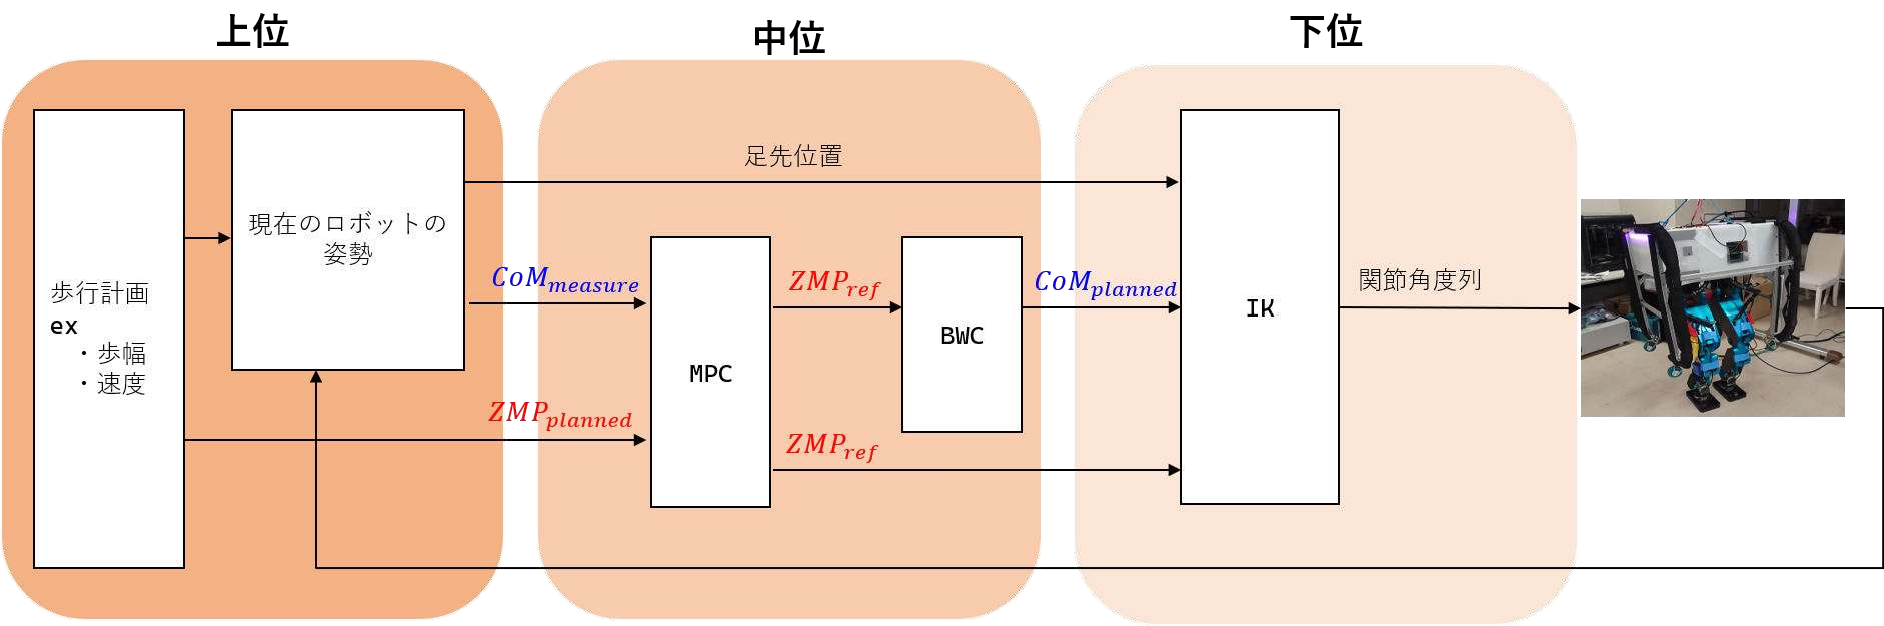
\includegraphics[width=1.0\linewidth]{images/control_flow.pdf}
  \caption{二足歩行ロボットの制御フロー}
  \label{fig:control_flow}
\end{figure}


\section{重心（CoM）に基づく歩行制御の考え方}

重心（CoM）は，ロボット全体の質量分布を代表する点として定義される．二足歩行ロボットにおいては，多数のリンクと関節から構成される全身の運動を直接扱うことは複雑であるため，CoMの運動に着目して歩行の安定性を議論する手法が広く用いられている．

歩行中のロボットの安定性は，CoMの位置や加速度が床反力とどのような関係にあるかによって特徴づけられる．特に，CoMの水平方向の運動は，転倒方向や支持脚への負荷分布に大きく影響する．このため，多くの歩行制御手法では，CoMの目標軌道を生成し，それに追従させることが基本的な方針となっている．

一方で，CoMの鉛直方向の運動は，水平方向に比べて制御対象として明示的に扱われない場合が多い．これは，従来のモデルではCoM高さを一定と仮定することで，問題を簡略化してきたためである．しかし，実環境においては，床の変形や沈み込みによって，CoM高さが変動する状況が生じる．この点については，第4章以降で詳しく議論する．

\section{ZMPと支持多角形による安定性評価}

二足歩行ロボットの安定性を評価する代表的な指標として，ZMP（Zero Moment Point）が広く用いられている．ZMPとは，床反力によるモーメントがゼロとなる床面上の点であり，この点が支持多角形の内部に存在する場合，ロボットは転倒しないと考えられる．

支持多角形は，ロボットが床と接触している支持脚の接地点を結んで形成される領域である（\cref{fig:foot_shape}）．両脚支持期（Double Support: DS）では支持多角形は広く，片脚支持期（Single Support: SS）では支持多角形は支持脚足裏の領域に限定される．このため，SSでは安定性の余裕が小さく，制御がより困難となる．

ZMPは，CoMの運動と密接に関係しており，CoMの加速度や高さの変化によってその位置が変動する．したがって，ZMPを支持多角形内に保つことは，CoM運動を適切に制御することと等価であると捉えることができる．

\begin{figure}[htbp]
  \centering
  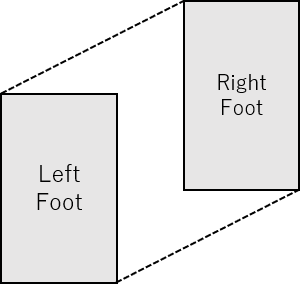
\includegraphics[width=0.3\linewidth]{images/foot.png}
  \caption{支持多角形}
  \label{fig:foot_shape}
\end{figure}

\section{線形倒立振子モデル（LIPM）の概要}

線形倒立振子モデル（LIPM）は，二足歩行ロボットの歩行制御において広く用いられている簡略化モデルである．LIPMでは，ロボットの全質量が一点のCoMに集中していると仮定し，そのCoMが一定の高さで運動する倒立振子としてモデル化される．また，角運動量の影響を無視することで，CoMの水平方向運動とZMPの関係を線形な形で記述できる．

このモデルにより，ZMPを入力としてCoM運動を解析・設計することが可能となり，歩行生成や安定化制御が大幅に簡略化される．一方で，CoM高さが一定であるという仮定は，床が剛体であることを前提としており，床の変形や沈み込みが生じる状況では必ずしも成立しない．

LIPMは実用上非常に有用なモデルであるが，その仮定と適用範囲を理解したうえで使用する必要がある．本研究では，この仮定が破綻する状況として，軟弱地面における歩行を対象とする．

\section{CoM制御の役割と本研究における位置づけ}

歩行制御におけるCoM制御は，歩行生成と安定化制御をつなぐ中核的な役割を担っている．上位層で生成されたCoM参照軌道に基づき，実際のCoM運動を調整することで，ZMPを支持多角形内に保ち，歩行の安定性を確保する．

従来の多くの手法では，CoMの水平方向の運動制御に主眼が置かれており，鉛直方向の運動は一定もしくは単純な関数として扱われてきた．しかし，床が変形する環境では，CoM高さの変動がZMPや床反力分布に影響を及ぼし，歩行安定性を低下させる要因となる．

本研究では，この点に着目し，床沈み込みに応じてCoM高さ参照を調整することで，歩行安定性を向上させる手法を検討する．本章で述べた基礎概念を踏まえ，次章では既存研究における歩行制御手法とその課題について整理する．